\documentclass[11pt]{article}            % Report class in 11 points
\parindent0pt  \parskip10pt             % make block paragraphs
\usepackage{graphicx}
\usepackage{listings}
\newcommand\tab[1][1cm]{\hspace*{#1}}
\usepackage{float}
\usepackage[document]{ragged2e}
\graphicspath{ {images/} }
\usepackage{graphicx} %  graphics header file
\begin{document}
\begin{titlepage}
    \centering
  \vfill
    
\includegraphics[width=8cm]{uni_logo.png} \\ 
	\vskip2cm
    {\bfseries\Large
	Data Structure and Algorithm \\ (CS09203)\\
	
	\vskip2cm
	Lab Report 
	 
	\vskip2cm
	}    

\begin{center}
\begin{tabular}{ l l  } 

Name: & Muhammad Umer \\ 
Registration \#: & CSU-F16-104 \\ 
Lab Report \#: & 01 \\ 
 Dated:& 26-03-2018\\ 
Submitted To:& Mr. Usman Ahmed\\ 

 %\hline
\end{tabular}
\end{center}
    \vfill
    The University of Lahore, Islamabad Campus\\
Department of Computer Science \& Information Technology
\end{titlepage}


    
    {\bfseries\Large
\centering
	Experiment \# 2 \\

Queue with Array implementation\\
	
	}    
 \vskip1cm
 \textbf {Objective}\\ The objective of this session is to understand the various operations on queues using array structure in C++.\\~\\
 \textbf {Software Tool} \\
1.  Window 7 (32-bit)\\
2. Sublime Text Editor\\
3. Dev C++

\textbf{Theory }

\textbf{Queue using Array:-}\\
This manual discusses an important data structure, called a queue. The idea of a queue in
computer science is the same as the idea of the queues to which you are accustomed in
everyday life. There are queues of customers in a bank or in a grocery store and queues of cars
waiting to pass through a tollbooth. Similarly, because a computer can send a print request faster
than a printer can print, a queue of documents is often waiting to be printed at a printer. The
general rule to process elements in a queue is that the customer at the front of the queue is served
next and that when a new customer arrives, he or she stands at the end of the queue. That is, a
queue is a First In First Out data structure.\\~\\
A queue is a set of elements of the same type in which the elements are added at one end, called
the back or rear, and deleted from the other end, called the front. For example, consider a line
of customers in a bank, wherein the customers are waiting to withdraw/deposit money or to
conduct some other business. Each new customer gets in the line at the rear. Whenever a teller
is ready for a new customer, the customer at the front of the line is served.\\~\\
The rear of the queue is accessed whenever a new element is added to the queue, and the front
of the queue is accessed whenever an element is deleted from the queue. As in a stack, the
middle elements of the queue are inaccessible, even if the queue elements are stored in an array.\\~\\
Queue: A data structure in which the elements are added at one end, called the rear, and deleted
from the other end, called the front; a First-In-First-Out (FIFO) data structure.\\~\\
Queues may be represented in the computer in various ways, usually by means at one-way list
or linear arrays. Unless otherwise stated or implied each of our queues will be maintained
by a linear array QUEUE and two pointer variable FRONT containing the location of the
front element of the queue and REAR containing the location of the rear element of the queue.
The condition FRONT = NULL will indicate that the queue is empty.\\~\\
\begin{figure}[H]
\centering
  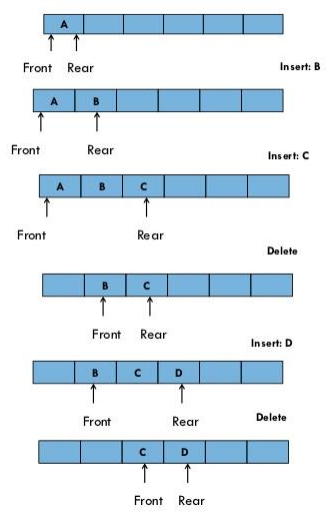
\includegraphics[width=12cm,height=10cm,keepaspectratio]{1.png}
\caption{}
\label{}    
\end{figure}

Whenever an element is deleted from the queue the value of FRONT is increased by one.
This can be implemented by the assignment.
\begin{center}	FRONT = FRONT + 1 \end{center}
Similarly, whenever an element is added to the queue the value of REAR is increased by
one. This can be implemented by the assignment.
\begin{center}		REAR = REAR + 1 \end{center}
This means that after N insertions the rear element of the queue will occupy QUEUE [N] or in
other words eventually the queue will occupy the last part of the array. This occurs even though
the queue itself may not contain many elements.\\~\\
Suppose we want to insert an element ITEM into a queue at the time the queue does occupy
the last part of the array i.e. when REAR = N. One way is to do this simply move the entire
queue to the beginning of the array changing FRONT and REAR accordingly, and then inserting
ITEM as above. This procedure may by very expensive. The procedure we adopt is to assume
that the array QUEUE is circular that is that QUEUE [1] comes after QUEUE [N] in the array.
With this assumption, we insert ITEM into the queue by assigning ITEM to QUEUE [1].
Specifically, instead of increasing REAR to N+1 we reset REAR=1 and then assign
\begin{center}	QUEUE[REAR] = ITEM \end{center}
Similarly, if FRONT=N and an element is deleted then we reset FRONT=1 instead of
increasing
\begin{center}		FRONT to N+1. \end{center}
Suppose that our queue only contains one element i.e. suppose that
\begin{center}	FRONT = REAR ≠ NULL \end{center}
And suppose that the element is deleted. Then we assign FRONT = NULL and REAR
= NULL to indicate that the queue is empty.\\~\\~\\


\textbf{Algorithm for insertion:-}\\
QINSERT (QUEUE, N, FRONT,REAR, ITEM)\\
This procedure inserts an element ITEM into a queue.\\
\tab	1.[Queue already filled?]\\
If FRONT = 1 and REAR = N or if FRONT =REAR+1 then\\
Write OVERFLOW and Return.\\
\tab	2.[Find new value of REAR]\\
If FRONT = NULL then [Queue initially empty] Set FRONT =1\\
and REAR = 1.\\
\tab 	else if REAR = N then\\
Set REAR = 1.\\
else\\
Set REAR = REAR + 1. [End of if Structure]\\
3.Set QUEUE[REAR] = ITEM [This insert new element]\\
4.Return.\\~\\

\textbf{Algorithm for Deletion from Queues:-}\\
QDELETE (QUEUE , N ,FRONT REAR, ITEM)\\
This procedure deletes an element from a queue and assigns it to the variable ITEM.\\~\\
1.[Queue already empty?]\\
If FRONT = NULL then Write Underflow and Return.\\
2.Set ITEM = QUEUE[FRONT]\\
3.[Find new value of FRONT]\\
If FRONT = REAR then [Queue has only one element to start]\\
Set FRONT = NULL and REAR = NULL\\
\tab else if FRONT = N then\\
Set FRONT = 1\\
else\\
\tab Set FRONT = FRONT + 1 [End of If Structure]\\
4.Return.\\~\\

\textbf{Lab Task:-}\\
Write a C++ code to perform insertion and deletion in queue using arrays applying
the algorithms given in the manual. Create a menu shown below.\\
\begin{figure}[H]
\centering
  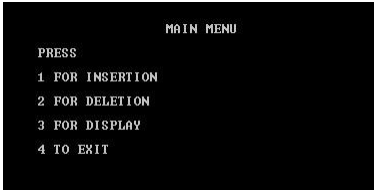
\includegraphics[width=12cm,height=6cm,keepaspectratio]{2.png}
\caption{The ouput of the program}
\label{Figure:1}    
\end{figure}


\textbf{Solution:-}\\~\\
\begin{lstlisting}[language=C++]
#include<iostream>
#include<conio.h>
using namespace std;

void insert(int queue[], int n, int& front, int& rear){
	int item;
	if((front == 1 && rear == n) || front == rear + 1){
		cout<<"\n\nError: Queue Overflow!";
		cout<<"\n\nPress any key to continue....";
		getch();
		return;
	}
	cout<<"\n\nEnter a value: ";
	cin>>item;
	if(front == 0){
		front = 1;
		rear = 1;
	}
	else if(rear == n)
		rear = 1;
	else
		++rear;	
	queue[rear] = item;
	cout<<"\n\nValue inserted Successfully";
	cout<<"\n\nPress any key to continue....";
	getch();
}

void deletion(int queue[], int n, int& front, int& rear){
	if(front == 0){
		cout<<"\n\nError: Queue Underflow!";
		cout<<"\n\nPress any key to continue....";
		getch();
		return;
	}
	int item;
	item = queue[front];
	if(front == rear){
		front = 0;
		rear = 0;
	}
	else if(front == n)
		front = 1;
	else
		front++;
	cout<<"\n\nValue deleted Successfully";
	cout<<"\n\nPress any key to continue....";
	getch();
}

void display(int queue[], int n, int& front, int& rear){
	if(front == 0 && rear == 0){
		cout<<"\n\nQueue is Empty!\n\n";
		cout<<"\n\nPress any key to continue....";
		getch();
		return;
	}
	cout<<"\n\nItems in the queue\n\n";
	for(int i=front; i<=rear; i++){
		cout<<queue[i]<<" ";
	}
	cout<<"\n\nPress any key to continue....";
	getch();
}

int main()
{
	int choice, n = 15, queue[n], front = 0, rear = 0,value;
	up:
	system("cls");
	cout<<"\t\t\tMAIN MENU\n\n";
	cout<<"\tPRESS\n\n";
	cout<<"\t1 FOR INSERTION\n\n";
	cout<<"\t2 FOR DELETION\n\n";
	cout<<"\t3 FOR DISPLAY\n\n";
	cout<<"\t4 TO EXIT\n\n";
	cout<<"PLEASE ENTER YOUR CHOICE\n\n";
	cin>>choice;
	if(choice == 1){
		insert(queue, n, front, rear);
		goto up;
	}
	else if(choice == 2){
		deletion(queue, n, front, rear);
		goto up;
	}
	else if(choice == 3){
		display(queue, n, front, rear);
		goto up;
	}
	else if(choice == 4)
		exit(0);
	else{
		cout<<"\n\nWRONG CHOICE!";
		cout<<"\n\nPRESS ANY KEY TO CHOOSE AGAIN...";
		getch();
		goto up;
	}
	return 0;
}
\end{lstlisting}

\textbf{Output:-}
\begin{figure}[H]
\centering
  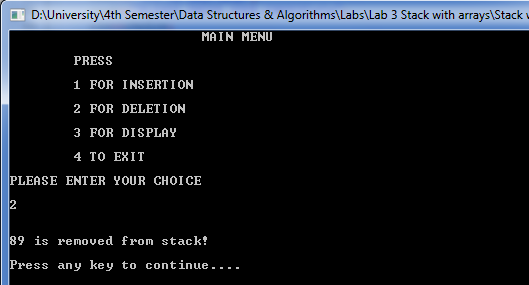
\includegraphics[width=12cm,height=6cm,keepaspectratio]{3.png}
\caption{Main menu and insertion operation}
\label{Figure:3}    
\end{figure}

\begin{figure}[H]
\centering
  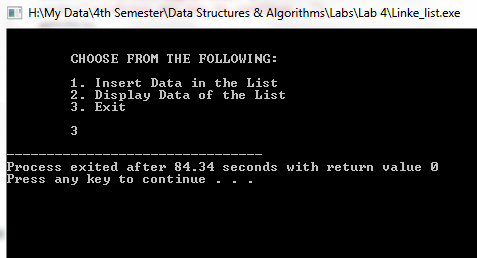
\includegraphics[width=12cm,height=6cm,keepaspectratio]{4.png}
\caption{Displaying after insertion}
\label{Figure:4}    
\end{figure}

\begin{figure}[H]
\centering
  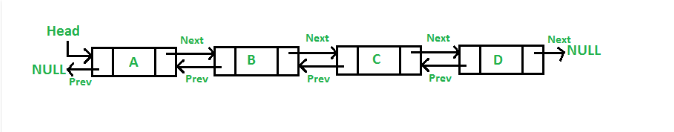
\includegraphics[width=12cm,height=6cm,keepaspectratio]{5.png}
\caption{Deleting operation}
\label{Figure:5}    
\end{figure}

\begin{figure}[H]
\centering
  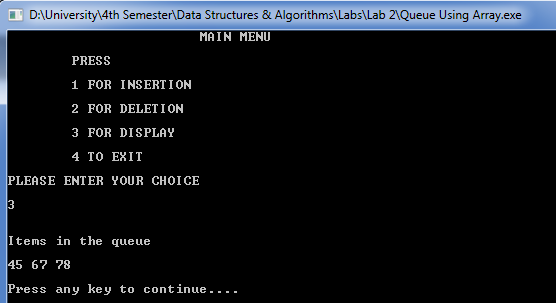
\includegraphics[width=12cm,height=6cm,keepaspectratio]{6.png}
\caption{Displaying after deletion}
\label{Figure:6}    
\end{figure}

\begin{figure}[H]
\centering
  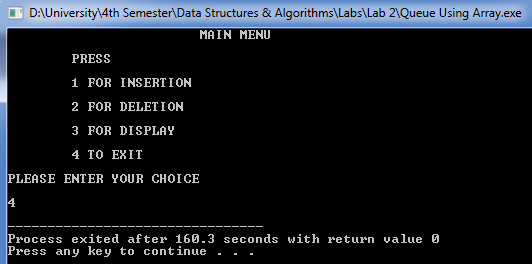
\includegraphics[width=12cm,height=6cm,keepaspectratio]{7.png}
\caption{Exit}
\label{Figure:7}    
\end{figure}

\textbf{Source Code:-}
https://github.com/umerayan/Semester-4-Labs.git\\~\\

\textbf{Conclusion:-}
Queue in computer science is same as we accustomed in everyday life. There are many examples of queue in everyday life i.e. in Banks, grocery store, and queues of cars waiting to pass through a tollbooth.
In computers one of the best example of queues that computer sends a print request to the printer in a queue page by page.A queue is a First in First out data structure.\\~\\
We implemented the queue program using the algorithm given in the manual. The program performs the every task related to queue in daily life or in computer. This program can be use to understand and fulfill the problem of queue in your software.
The program is coded in C++ language and open source for everyone at my guthub account (The link mentioned above).\\~\\~\\

\tab[6cm] \noindent\rule{6cm}{0.4pt}\\
\tab[6cm] (Concerned Teacher/Lab Engineer)
 
\end{document}                          % The required last line
